%!TEX root = thesis.tex
\chapter{Methods}
\label{chap:methods}

overview of the methodology to be used;

\section{Sensor observation service}
Retrieve sensor metadata from the sensor observation service. There are a number of different requests that can be made: GetCapabilities, DescribeSensor and GetObservation. These requests can be made as a \ac{http} GET request or a \ac{http} POST request. The response is an \ac{xml} document using the \ac{om} (for GetObservation) or \ac{sensorml} (for DescribeSensor).

\section{Resource description framework}
Publishing static geographic data on the semantic web requires a conversion of Shapefile to \ac{rdf}. First the Shapefile is loaded into a Postgis database. After that a Python script retrieves the records from the database, maps it to an ontology and writes it to an \ac{rdf} file. The final step is to publish the \ac{rdf} online \citep{LD:Missier}. 

The sensor metadata is also being published on the semantic web. To do this an \ac{xml} document is automatically retrieved from a \ac{sos} by a Python script. This script then extracts the relevant data from the \ac{xml} and maps it to an ontology. It outputs an \ac{rdf} file that will be published online. When new sources of sensor data are added the \ac{rdf} document will be updated.   

\section{Ontology mapping}
To publish data on the semantic web ontologies are required to specify the different classes and their relations. An ontology for static geographic data has to be connected to an ontology for sensor metadata. For this the ontologies by \cite{SSW:Cox4} will be used (\ac{owl} for observations and \ac{owl} for sampling features) in combination with the GeoSPARQL vocabulary for geometries as linked data \citep{LD:OGC}. The \ac{uml} diagram (figure \ref{fig:UML}) describes different components of \ac{om} observations in relation to sampling features and to the \ac{iso} standards 'general feature' and 'general feature instance'.  

\begin{figure}
	\centering
	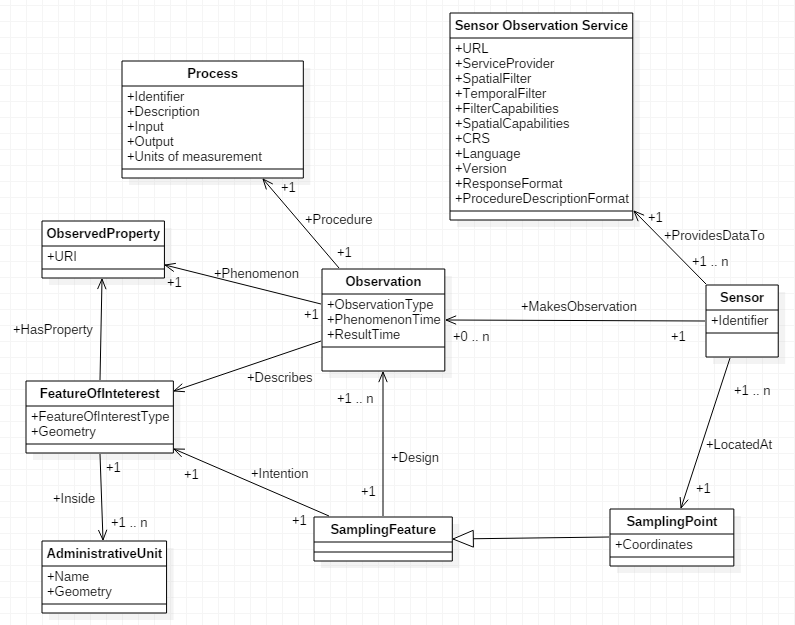
\includegraphics[width=1\linewidth]{figs/UML_Diagram.png}
	\caption{\ac{uml} diagram of observations based on \cite{SSW:Cox3}}
	\label{fig:UML}
\end{figure}

\section{Sensor data aggregation}
There are many different ways to aggregate sensor data, for example by taking the minimum value, the maximum value, the average value, the sum, etc. In order to determine which method of aggregation is applicable for a specific kind of sensor data the sensor metadata will contain links to appropriate aggregation methods. However, which methods are appropriate should be based on expert knowledge. Therefore, this requires a literature analysis. 


\iffalse

A \ac{wps} will be used for sensor data aggregation, including methods as minimum, maximum, mean and sum, but also temporal aggregation. 


\section{Standards}
\subsection{Sensor Web Enablement}
\ac{sos} and \ac{ssn}

\subsection{Semantic Web}

\begin{itemize}
	\item Store \ac{osm} data: create \ac{rdf} on-the-fly to prevent double storage. 
	\item Retrieve sensor metadata: create \ac{rdf} from \ac{om} which is returned by \ac{sos} getCapabilities/describeSensor requests
	\item Use \ac{ssn} as ontology for semantic sensor metadata 
	\item Use \ac{owl} as language for storing semantic \ac{rdf} triples
\end{itemize}


Query metadata: SPARQL, geo-SPARQL or stSPARQL? and which query engine?

\section{Ontologies}
The \ac{om} ontology is retrieved from sensors\\
Use \ac{ssn} ontology ontology to store metadata from sensors.  

\section{Middleware}
Creating own middleware to link sensors semantically and retrieve aggregated data\\

\ac{rest}ful service

\begin{figure}
	\centering
	\includegraphics[width=2\linewidth, angle=90]{figs/flowchart.png}
	\caption{Flow chart showing the differen components of the implementation}
	\label{fig:Flowchart}
\end{figure}
\fi




